% !TeX spellcheck = en_GB
\begin{wrapfigure}[19]{r}{0.44\textwidth}
	\vspace{-\normalbaselineskip}
	\centering
    \begin{subfigure}[b]{0.4\textwidth}
    	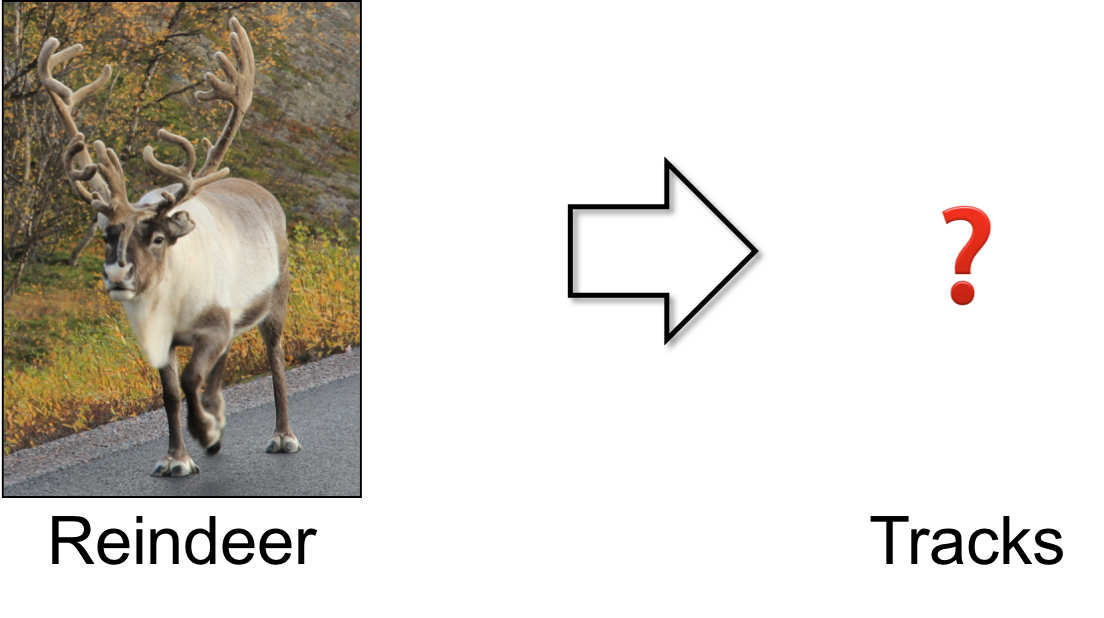
\includegraphics[trim={0cm, 0cm, 0cm, 0cm},clip,width=\textwidth]{./fig_instruments/Forward_problem.png}
        \caption{Forward problem.}\label{fig:dragon:forward}
    \end{subfigure}
    
    \begin{subfigure}[b]{0.4\textwidth}
    	
\includegraphics[trim={0cm, 0cm, 0cm, 0cm},clip,width=\textwidth]{./fig_instruments/Inverse_problem.png}
        \caption{Inverse problem.}\label{fig:dragon:inverse}
    \end{subfigure}
\caption{\protect\subref{fig:dragon:forward}: Relationship between parameter of interest (reindeer) and the unknown parameter of measurements (tracks). \protect\subref{fig:dragon:inverse}: Inverse problem when the parameter of measurements is known but the parameter of interest is not \citep{stephens_remote_1994}.}\label{fig:dragon}
	\vspace{-\normalbaselineskip} 
\end{wrapfigure}

